\chapter{引言}
\section{研究背景和意义}
地震勘探的终极目标是通过观测到地震数据来定量地估计地下模型。
弹性参数,包括纵(P)波速度,横(S)波速度以及密度等等物性参数可以通过岩石物理来定量的估计岩石物理参数,从而获得储层及其围岩的岩石性质。这对油气的开发,油田
监测以及CO$_2$注入等具有重要意义。传统的常规地震数据处理中,通常用声波方程来描述地震波在地下介质中的传播。而地下介质的真实模型往往要复杂得多,需要通过弹性
各向同性、具有垂直(水平)对称轴的横向各向同性(VTI,HTI)、正交各向异性(ORT)、衰减等等来更准确的描述波传播。但是模型假设越复杂,所引入的计算量也越大,
而所对应的多参数反问题也越困难。目前来看从声介质过渡到弹性介质能够以较小代价来获取较准确的模型近似。
尽管如此,从声波近似过渡到到弹性假设也会成倍地增加计算量,但是采用弹性波假设来进行成像或者反演仍然十分必要。因为考虑弹性假设的数据处理流程能区分数据中的
P波与S波模式,从而获得更多与岩性相关的信息,这对于岩性估计、流体识别、气云成像、裂缝与应力刻画以及密度估计都非常重要。
近年来,非常规油气藏,如致密页岩气(油)等开发技术极大地依赖于岩石物理参数的估计,这使得考虑弹性介质甚至各向异性假设都需要提上日程。

地震勘探中的诸多技术都非常依赖于速度模型的精度。
因此在众多物性参数中,如何获取准确的高分辨率速度模型是地震勘探中最为迫切的任务。
为了降低地震数据与模型描述之间的非线性程度,Claerbout(1985)\cite{Claerbout1985Imaging}在其书中将速度模型分解为两个部分:1)描述速度(阻抗)界面的高频部分;
2)描述波传播走时的低频部分。这样的分解方式分别对应于地震勘探中最核心的两个任务,也即偏移成像与速度建模。传统方法中偏移成像+AVO/AVA
技术通常用来获取模型的高频部分,
而偏移速度分析(MVA)和层析技术被用来恢复模型的低频部分。但是这类方法所能恢复的波数谱上存在明显的间断区域,正如著名的图\ref{fig:GapInSeisVel}
所示(选自Claerbout(1985)\cite{Claerbout1985Imaging}),速度模型的中低成分波数很难恢复。这就需要引入旨在恢复全频带速度信息的FWI方法。
而随着高性能计算能力的不断提升,基于波动理论来获取模型高、低波数成分的方法也受到了广泛关注。
\begin{figure}[!htb] 
   \centering 
   \subfloat[]{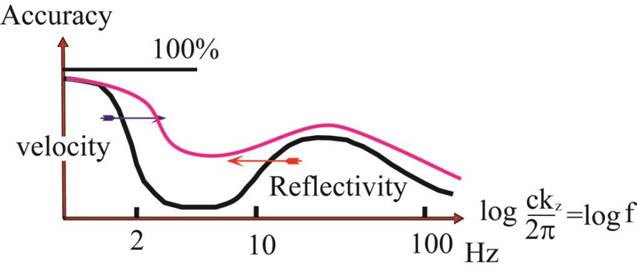
\includegraphics[width=0.68\textwidth]{Figure/chapter01/GapInSeis.jpg}}
   \caption{Vertical profiles of elastic WERTI and EFWI results at 1.4km (a) and
       3km (b). The black and blue lines indicate the true and linearly         increased
       initial model. The green and yellow lines indicate the WERTI and EFWI    results,
       respectively.
   }
   \label{fig:GapInSeisVel}
\end{figure}

传统常规方法中大多基于射线类方法进行成像与速度估计,这在模型复杂区域很难处理多路径以及焦散等问题。而基于波动方程的方法则可以避免上述问题。
目前基于波动理论的主要反演方法主要有以下三类:

1、FWI,该方法通过匹配数据中携带的所有信息,包括走时、振幅、模式转换、多次波等等,来获得对地下模型的全波数谱的
恢复。
相比走时反演和MVA,它可以获取更高分辨率的地下模型。
因此自从Lailly(1983)\cite{lailly1983seismic}和Taratola(1984)\cite{tarantola1984}建立了FWI理论框架之后,随着宽频带,宽方位数据采集的成熟,FWI
被认为是填补速度模型中尺度波数成分空白的最强有力的工具。
但是FWI也受到众多的制约,如强烈的非线性程度(cycle-skipping),数据不完备导致的有限观测孔径,地下实际介质的非弹性以及各向异性,计算代价十分昂贵等等,因此
FWI虽经过数十年发展所面临的挑战依然十分艰巨;

2、波动方程偏移速度分析(WEMVA),该类方法旨在更新模型中的长波长背景速度,也即模型的低波数成分。
目前主流的做法通常利用数据中的反射波信息,通过获取反射波波路径信息来获得模型中深部的速度更新。
而根据其目标函数的残差类型又可以分为数据域反演(如Xu et al., 2012\cite{xu:2012};Wu and Alkhalifah, 2015\cite[]{Wu2015}; Zhou et al, 
2015\cite[]{zhou:2015}; Chi et al, 2015\cite{chi:2015})和扩展成像域反演(如Sava和Fomel, 2006\cite{Sava2006}; Almomin和Biondi, 2012\cite{Almomin2012})。
此类方法与基于射线理论的成像域层析与数据域(非线性)层析方法一脉相承,但是避免了传统层析流程中繁琐的人工拾取工作,不过其同样也会受困于cycle-skipping等问题;

3、最小二乘逆时偏移(LSRTM),该方法可以看作是线性化的FWI,在初始模型足够好的时候通过匹配模拟数据与观测数据的振幅来获得地下反射系数模型。常规偏移成像
采用伴随算子来近似正传算子的伪逆,从而近似地获得反射率的成像结果。但是伴随算子通常近似效果很差,最小平方偏移(LSM)通过迭代方式来获取正传算子的伪逆从而获得
更好的成像效果((Nemeth et al., 1999,Kühl and Sacchi, 2003,Dai, 2012)。该过程可以看作是对目标函数对模型的二阶导数,也即Hessian,近似求逆的过程。

结合以上背景,如何恢复弹性介质中的速度模型将对勘探地球物理的发展至关重要。将弹性假设引入到以上反演问题中将会大大增加反问题的非线性程度。同时,多参数反演
也会带来参数间的耦合效应,这会进一步增加反演难度。由于计算机能力提升、多分量观测数据的增多以及解决声波FWI无法回避的问题的需要,考虑弹性甚至各向异
性的全波形反演逐渐成为研究热点。弹性波多分量数据中同时含有P波和S波,这两种不同波模式对地下介质有着不同的刻画作用。
近年来弹性波波模式分离技术能够提供准确的P或S波数据子集,这对反演中采取更多的多尺度策略带来可能性。在反演过程中,不同参数采用不同的数据子集或者不同的反演阶段
采用不同的数据子集,这将大大降低法多参数反演的非线性程度,同时也可以回避参数间的耦合效应。在本文中,这种策略将贯穿始终,
模式解耦将在EFWI,弹性波波动放程反射走时反演(EWERTI)以及E-LSRTM中提供的分离的P或S波数据,来帮助获得更好的反演结果。
\section{研究现状}
\subsection{弹性波FWI研究现状}
Claerbout(1971\cite{Claerbout1971})采用爆炸发射面的概念解释了成像条件可以通过多次叠加来对地下构造进行刻画。Lailly(1983\cite{lailly1983seismic})
和Tarantola(1984\cite{tarantola1984})最早引入了表示观测数据与模拟数据间波形残差的$L_2$目标函数,将这种偏移成像的原理重新转化为寻优的
最优化问题,也即FWI。而该最优化问题的梯度方向可以采用共轭状态法求取,通过入射波场与反传波场之间的互相关来获得。FWI试图将速度宏观模型的恢复(速度
建模)与偏移成像两个任务统一在一个流程中,这样就可以在地下每个网格点获得具有连续波数谱的高分辨率结果。但是早期只利用反射数据的FWI很少有令人满意的
结果,因为短偏移距观测的地震数据对中尺度波长的模型信息非常不敏感(Virieux和Operto(2009)\cite{virieux2009overview}),这就需要在初始模型非常准确
的时候FWI才能获得收敛。
从上世纪80年代末期,随着FWI在长偏移距以及井间透射波的应用成功,人们才发现FWI的潜力(Mora, 1987\cite{mora:1987}, 1988\cite{mora1988elastic}; Pratt
and Worthington, 1990\cite{PRATTEtAl1990}, Pratt et al., 1996\cite{pratt1996two})。
近年来在长偏移距、宽方位和宽频带采集的数据逐渐增多后,基于声波近似的FWI也在越来越多的实际数据中获得成功应用,例如Ravaut
et al., 2004\cite{RavautEtAl2004},Operto et al., 2006\cite{Operto2006},Shinet al.,
2009\cite{ShinEtAl2009}。然而即使对于含有长偏移距的数据而言,由于波传播路径的增加,非线性程度变得更加剧烈,因而从FWI中获得稳健的反演结
果仍然受到很大挑战\cite{sirgue2006importance,virieux2009overview}。

而从前文背景分析可以知道,最早始于Tarantola(1986)\cite{tarantola:1986}和Mora(1987)\cite{mora:1987}的弹性波全波形反演能够从多分量数据中反演地下介质的弹性参数,如P/S-波速度和密度。
尽管其仍然需要很大计算代价,EFWI还是在很多实际数据中获得了应用
\cite{crase1992nonlinear,djikpesse.tarantola:1999,sears:2008,sears:2010,prieux:2013a,prieux:2013b,vigh:2014}。
EFWI的实现方式可以在时间域\cite{shipp:2002},可以在频率域\cite{brossier2009},也可以采用混合的方式在时间域进行正演模拟而在频率域求解
\cite{nihei.li:2007,sirgue:2008}。然而,EFWI中多个参数参与反演会增加反问题的非线性程度,同时也会受到由于不同物理参数之间的串扰带来的反演
中参数耦合的影响\cite{forgues.lambare:1997}。在海洋环境中,尤其是在软海底环境中,由于P-to-
S的转换模式非常弱,基于拖缆或者海底多分量数据的EFWI的非线性程度会变得更严重\cite{sears:2008}。

从声波介质到弹性介质,波形反演方法将受到诸多挑战,解决EFWI中的问题,不仅要应对原有声波框架下的困难,同时也要解决多参数反演带来新问题。总的来说,
EFWI将主要面临以下两个方面的挑战:

1、反演的非线性,也即Cycle-skipping。FWI是基于Born近似的理论框架导出的。在Born散射下,Miller et al\cite{miller:1987}基于ray+Born理论,
导出模型中散射点局部的波数矢量可以表达为:
%\begin{equation}
$    \mathbf{k}=\mathbf{k_s}+\mathbf{k_r}=\frac{\omega}{v}cos\frac{\theta}{2}\mathbf{n}$。
%    \label{eq:Modelwnb}
%\end{equation}
其中$\mathbf{k}$为照明矢量,$\mathbf{k_s}$和$\mathbf{k_r}$分别是震源端和检波点端的波场波数矢量,$v$为局部速度,$\theta$为散射角,
$\omega$为角频率,$\mathbf{n}$为$\mathbf{k}$方向的单位向量。由上式可以看出,低频和大孔径($\theta$)数据对于中低波数成分的恢复至关重要。
\begin{figure}[!htb] 
   \centering 
   \subfloat{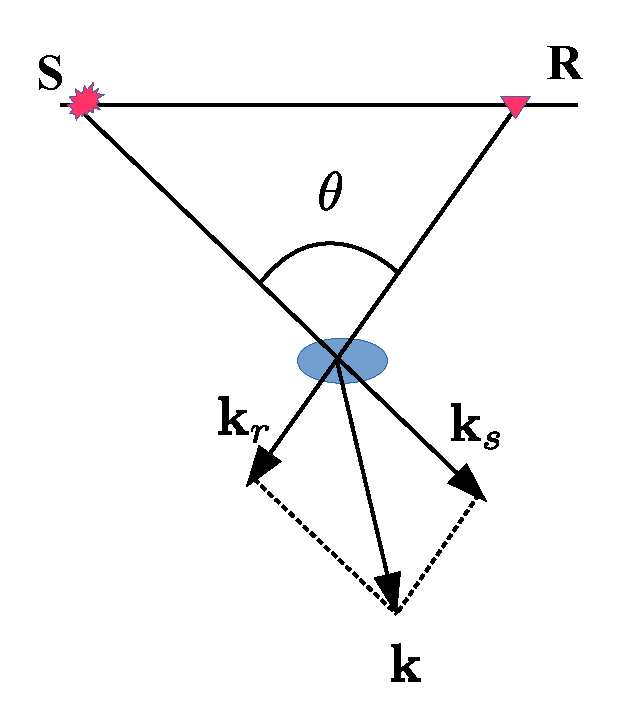
\includegraphics[width=0.40\textwidth]{Figure/chapter01/Wavenumbervector.pdf}}
   \subfloat{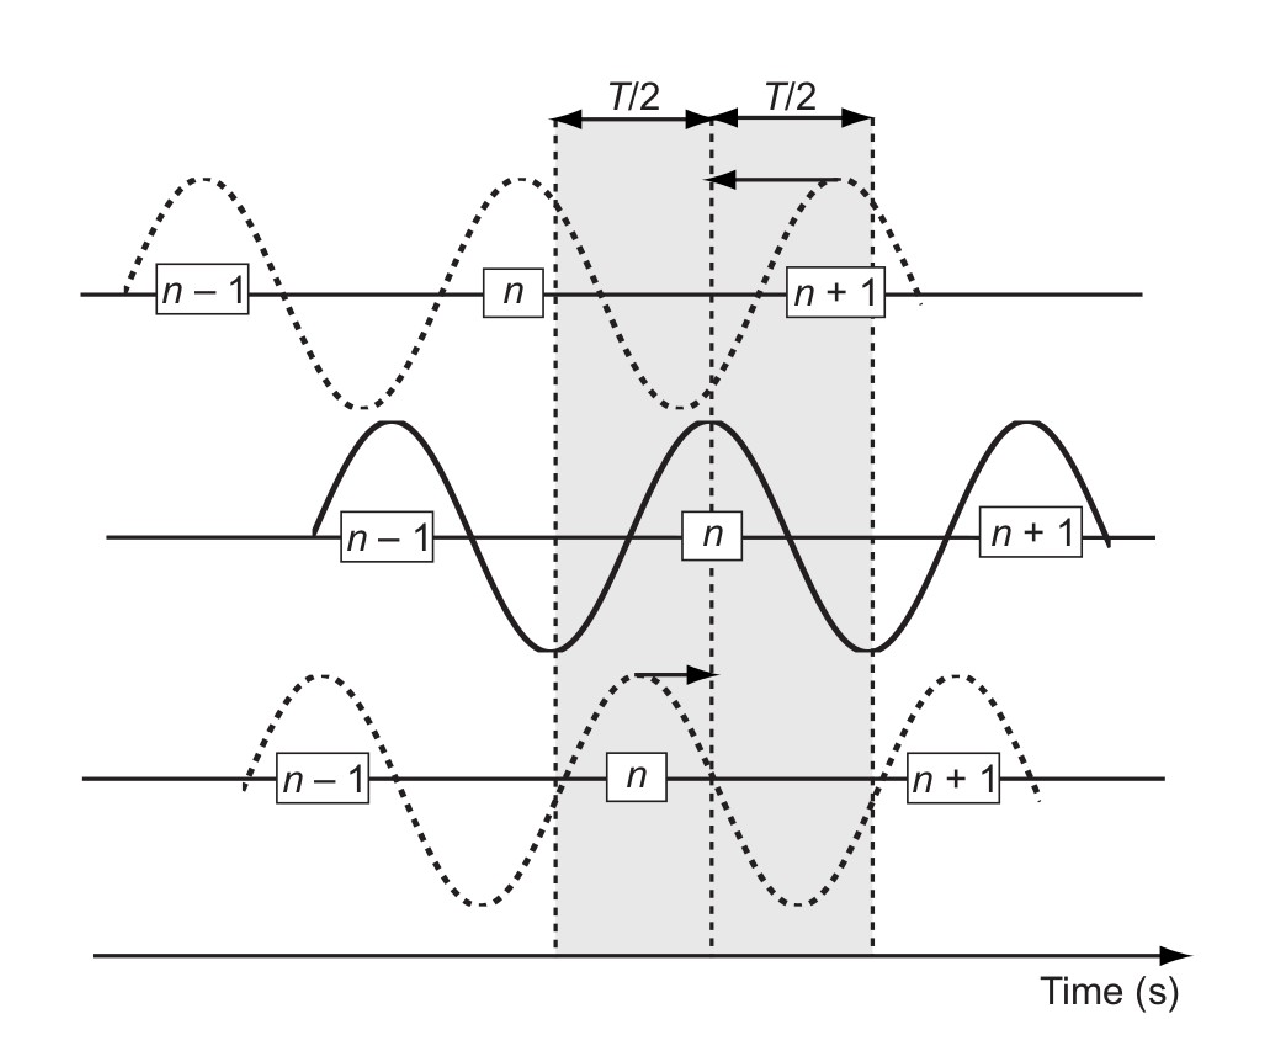
\includegraphics[width=0.40\textwidth]{Figure/chapter01/Cycle-skipping.pdf}}
   \caption{Vertical profiles of elastic WERTI and EFWI results at 1.4km (a) and
       3km (b). The black and blue lines indicate the true and linearly         increased
       initial model. The green and yellow lines indicate the WERTI and EFWI    results,
       respectively.
   }
   \label{fig:WavenumberVector}
\end{figure}
因此FWI的成功与否非常依赖于长偏移距记录和数据中有效的低频分量。如图\ref{fig:Cycle-skipping}
所示,如果初始模型不够好导致波形匹配时相差$\frac{1}{2}T$以上,那么就会使得反演陷入局部极值,这也就是所谓的“周波跳跃”问题。
在声波FWI中,发展了许多策略来解决非线性问题,如从低频到高频{\color{red}(Sirgue and Pratt, 2004; 刘国峰等, 2012; 刘璐等,2013; 曹书红和陈景波, 2014; 
张文生等, 2015),选取不同的时窗与偏移距逐步加入反演中(Shipp and Singh, 2002; Wang and Rao, 2009; Sears,2008),
修正目标函数使其凸性更好(Luo and Schuster, 1991;Tromp et al., 2005;Chi
et al., 2014; Wu et al., 2014; Shin and Cha, 2008; Luo et al., 2016;)}等等。这些策略可以用
在EFWI中,但是由于更多参数引入以及更复杂的弹性波波场,使得在使用这些策略的时候需要根据情况来择优选取。
而在EFWI中,不但会出现同样的强烈非线性,而且将面临更复杂的情况。
在构建初始模型的时候我们要同时获得足够好的$V_p$与$V_s$模型,这样才能对各种模式的转换波形进行
匹配。而$V_s$模型相比$V_p$初始模型更难获得。目前许多EFWI研究中都假设了$V_s$与$V_p$之间有着固定的Poisson's比值的关系,因此可以通过简单的系数相乘
来构建初始模型。但是当地下介质Poisson's比变化较大时很难获得较好的$V_s$初始模型,这就又增加了EFWI的困难。为了降低弹性波FWI非线性程度,许多学者通过
包络目标函数(黄超等,2015\cite{黄超2015},王官超和杜启振,2016\cite{王官超2016}),或者通过研究目标函数性态来指导多尺度策略的设计
(Brossier et al., 2010\cite{BrossierEtAl2010};王毓玮等,2016\cite{王毓玮2016})。
Tarantola(1986)\cite{tarantola:1986}指出EFWI应分主次顺序依次构建具有不同影响的参数。
或者采用多尺度策略多级的选取不同数据分量来进行反演(Sears, 2008\cite{sears:2008}; Operto et al., 2013
\cite{operto2013guided})。然而实际中,诸多因素会制约这些策略的应用,例如(低频缺失,初始模型不够好,子波估计,噪音等等)。因而降低EFWI的非线性
程度使得反演更加稳健可靠依然需要诸多努力。

2、多参数反演中的参数耦合效应。如果物理模型中引入多个参数,那么不同的参数扰动可能会引起类似的数据扰动。虽然其产生的数据扰动可能不完全一致,
但是不同参数的“偏导数波场\cite{pratt1998gauss}”会在特定角度范围内的重叠,这就导致无法简单地区分开数据扰动来自哪一种
参数扰动,从而引起参数间的耦合效应。这样的话,即使在初始模型足够好的时候也很难从数据扰动中恢复其相应的参数扰动。为了解决EFWI中的参数耦合问题,
许多学者通过调查散射模式或者Hessian算子来选取不同的参数化方式(Wu and Aki, 1985\cite{wu.aki:1985};Tarantola, 1986\cite{tarantola:1986};
Plessix and Cao, 2011\cite{plessix.cao:2011},Gholami et al, 2013\cite{gholami2013})。
当然最有效的就是考虑多参数Hessian算子的方法,用Hessian的信息来压制参数耦合的影响(Fichtner et al., 2001\cite{fichtner2011hessian};Operto et al.,
2013\cite{operto2013guided},Pan et al., 2015\cite{pan2015estimation};Yang et al.,
2016\cite{yang:2016})。然而由于Hessian计算所需代价太过于昂贵,即使在声波FWI也很难在大规模问题中获得应用。在EFWI中想要获得压制参数耦合的效果,就
需要在反演中包含对Hessian的非对角区块的近似。近期,在Hessian非对角区块的近似与利用方面,许多学者都将其应用到了EFWI中,例如Wang
et al.(2016)\cite{WangEtAl2016}采用块对角Hessian压制参数耦合,Pan et al(2017)采用Hessian-free
的方式采用l-BFGS的优化策略进行多参数反演,Wang and Cheng
(2017)\cite{Wang2017}指出模式解耦可以部分的利用Hessian非对角块来压制P波对$V_s$反演的干扰。而于此同时EFWI中,由于密度参数对数据不敏感,因此密度
的反演依然很难获得令人满意的结果。
\subsection{弹性反射波FWI研究现状}
尽管常规FWI在长偏移距,宽方位数据中有着令人满意的效果,但是在这种观测系统下,FWI主要利用了长偏移距透射波以及临界反射波所携带的信息来更新速度模型的
中长尺度波长的分量。由于FWI的成功非常依赖这种透射信息,就会使得FWI往往缺乏足够的大偏移距信息来更新模型中深部结构的中低波数成分。
这就导致在深部的区域,FWI往往只能更新来自反射数据的高波数成分(也即是最小平方偏移的过程)而很难更新中低波数成分。从图\ref{fig:WavenumberVector}
中也可以看出,在相同频率和速度下,深部的反演需要更大的角度覆盖才能确保足够的低波数照明,这也意味着要更大的偏移距。然而即使对
于目前宽方位长偏移距的采集技术也很难保证这样的覆盖,况且更长的偏移距也意味着更强的非线性\cite{sirgue2006importance,virieux2009overview}。

利用反射波信息可以更好的照明深部,通常可以在成像域或者数据域实现深部的速度更新。在成像域,该类方法通常被称为偏移速度分析(MVA),其主要利用拉平
共成像点道集作为收敛准则。
在实际生产中,通过射线走时层析来利用反射波信息更新中深部的背景速度已经是非常成熟的技术\cite{woodward1992,Meng
et al., 2004; Woodward et al., 2008;
Jones,2010}。其通过将道集上的剩余时差(或深度差)反投影到射线路径上来获得速度更新。不过射线层析经常需要进行许多人工干预,尤其是在每轮迭代中进行
成像剖面与成像道集的拾取。而且在构造复杂区域,射线高频渐近近似失效,使得走时层析很难获得成功。
基于波动理论的成像域MVA方法通常
需要引入扩展成像条件,通过最小化扩展道集上非零偏移距的能量来实现更新\cite{Sava &
Fomel 2006; Yang & Sava 2011; Almomin & Biondi 2012; Biondi
& Almomin 2012; Sun & Symes 2012; Lameloise et al.
2015}。尽管在二维应用中取得了不错的效果,但是这类方法主要缺陷是计算代价太过昂贵,尤其实在三维问题中,一方面偏移成像需要大量计算,
另一方面扩展成像条件的施加同样耗费极大。

\subsection{弹性波LSRTM研究现状}
et al.(2016)\cite{WangEtAl2016}采用块对角Hessian压制参数耦合,Pan et al(2017)采用Hessian-free
的方式采用l-BFGS的优化策略进行多参数反演,Wang and Cheng
(2017)\cite{Wang2017}指出模式解耦可以部分的利用Hessian非对角块来压制P波对$V_s$反演的干扰。而于此同时EFWI中,由于密度参数对数据不敏感,因此密度
的反演依然很难获得令人满意的结果。
\section{研究内容}
